\section{Results}

Current results include typical time series for quantities of interest. Namely steam demand, electric demand, and power produced by VRE. We have also generated synthetic data for grid demand and solar power using the \texttt{trainARMA} function in \texttt{RAVEN}. Thus the first step of the methodology from Baker et. al has been completed.

\begin{figure}[H]
 	\centering
 	\label{fig:grid-demand}
 	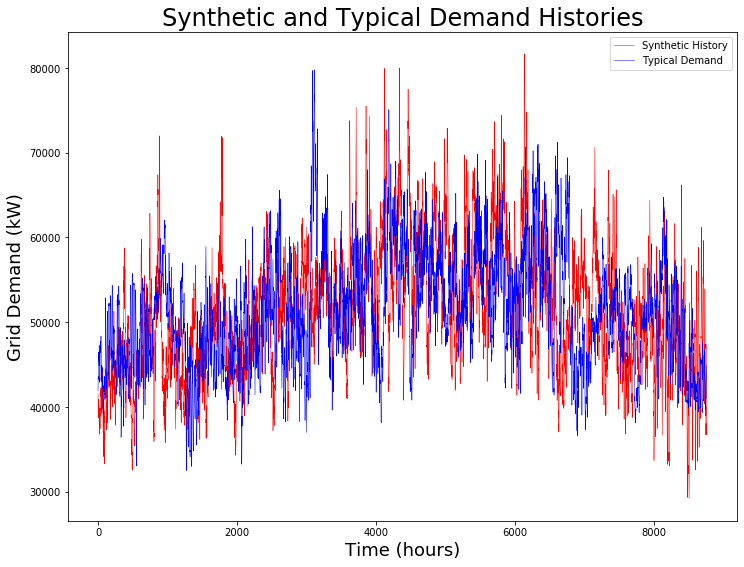
\includegraphics[width=0.8\columnwidth]{syn_vs_typ_hist.png}
 	\caption{The typical year of hourly grid demand in kW at UIUC.}
\end{figure} 
\begin{figure}[H]
	\centering
	\label{fig:steam-demand}
	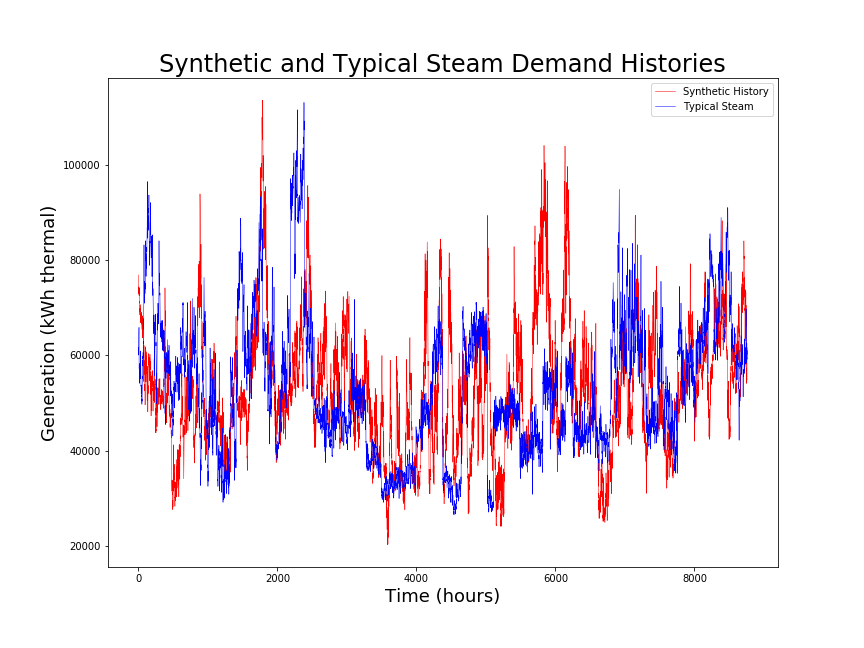
\includegraphics[width=0.8\columnwidth]{syn_vs_typ_steam.png}
	\caption{The typical year and a synthetic year of hourly steam demand in kW at UIUC.}
\end{figure}
\begin{figure}[H]
	\centering
	\label{fig:solar-power}
	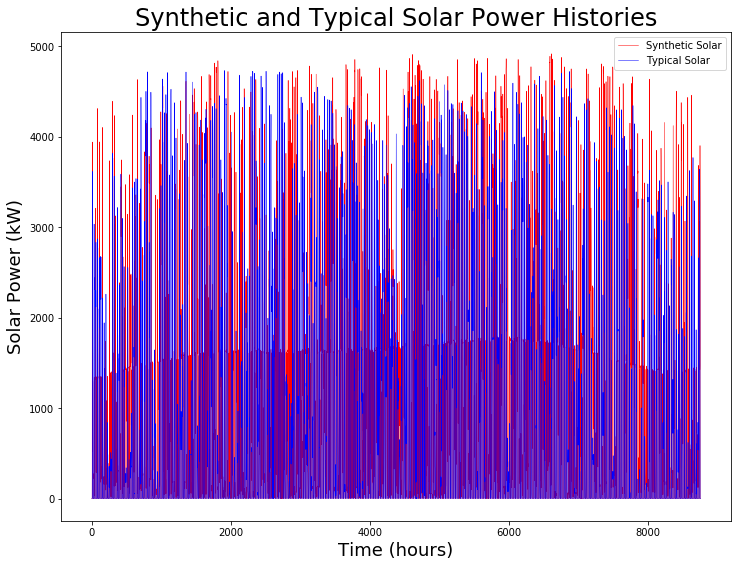
\includegraphics[width=0.8\columnwidth]{syn_vs_typ_sol.png}
	\caption{The typical year and a synthetic year of hourly power produced by the UIUC solar farm.}
\end{figure}
\begin{figure}[H]
	\centering
	\label{fig:wind-power}
	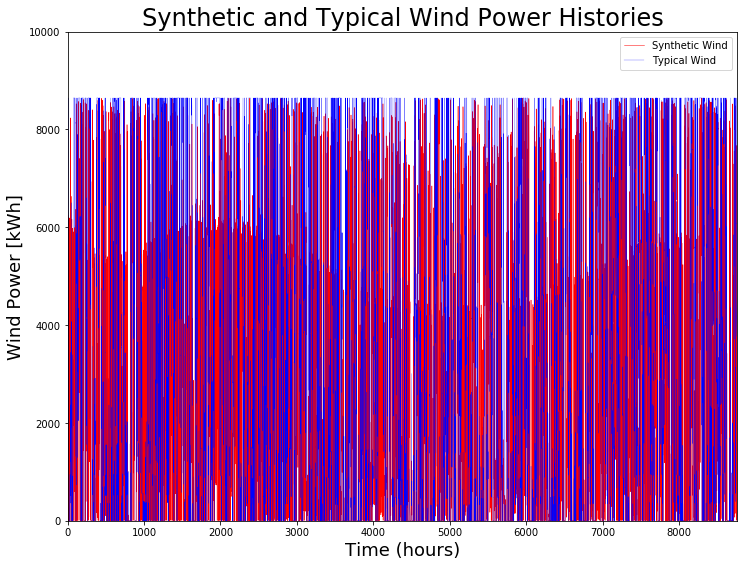
\includegraphics[width=0.8\columnwidth]{syn_vs_typ_wind.png}
	\caption{The typical year and a synthetic year of hourly wind power received by UIUC.}
\end{figure}